\documentclass{standalone}
\usepackage{tikz}
\usetikzlibrary{patterns, positioning}


\begin{document}
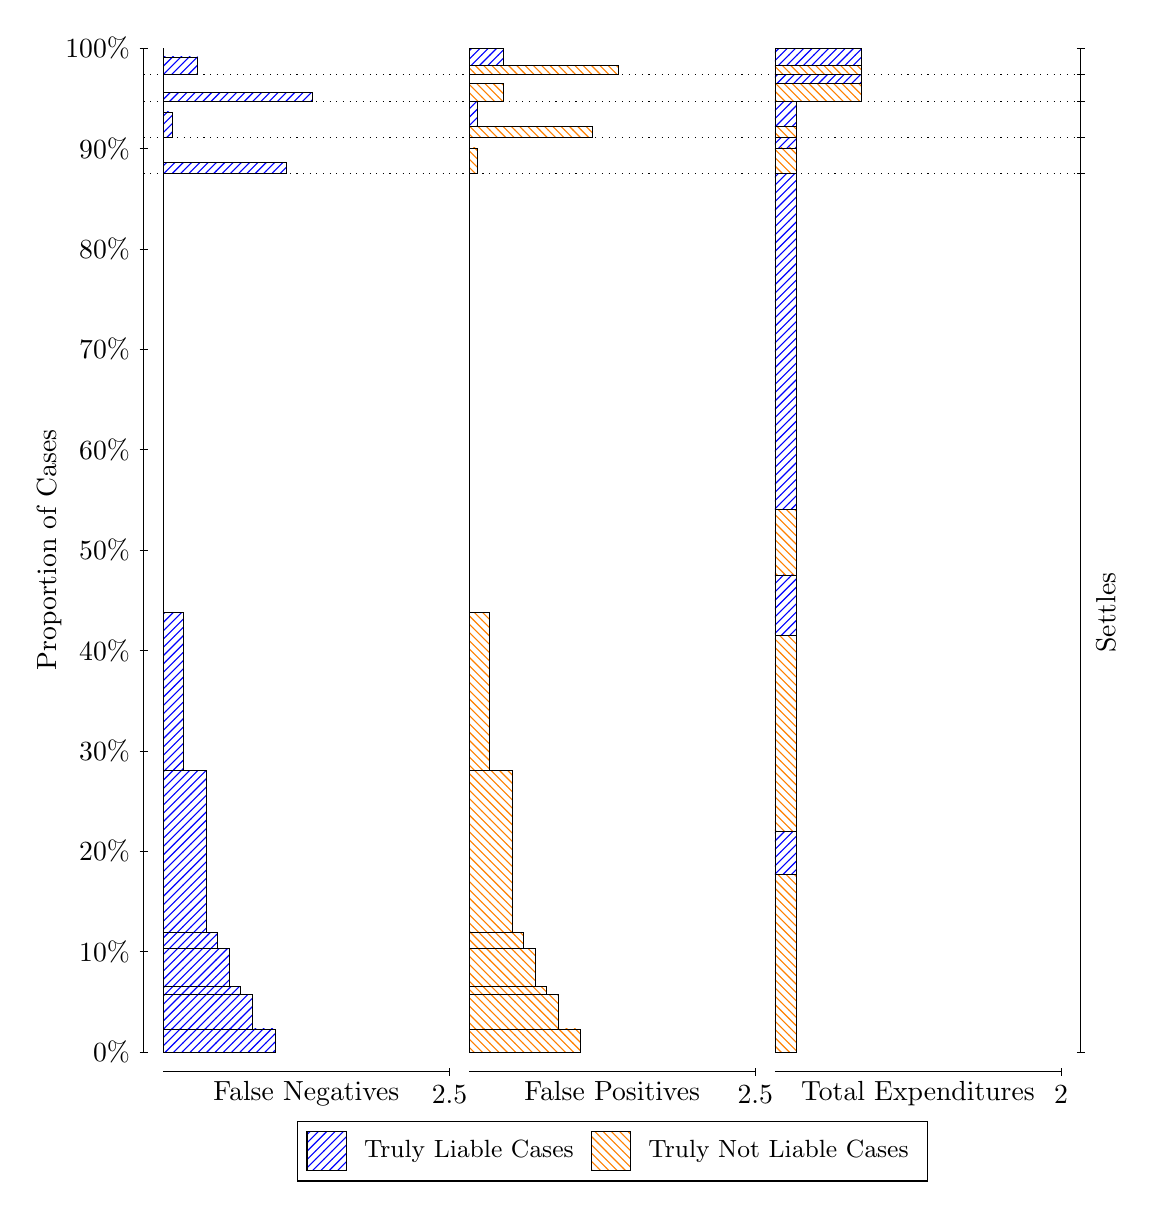
\begin{tikzpicture}
\draw[black, very thin] (1.5,1.75) -- (1.5,14.5);
\node[rotate=90, text=black, anchor=center] at (0.3, 8.125) {Proportion of Cases};
\draw[black, very thin] (1.45,1.75) -- (1.55,1.75);
\node[text=black, anchor=east] at (1.45, 1.75) {0\%};
\draw[black, very thin] (1.45,3.025) -- (1.55,3.025);
\node[text=black, anchor=east] at (1.45, 3.025) {10\%};
\draw[black, very thin] (1.45,4.3) -- (1.55,4.3);
\node[text=black, anchor=east] at (1.45, 4.3) {20\%};
\draw[black, very thin] (1.45,5.575) -- (1.55,5.575);
\node[text=black, anchor=east] at (1.45, 5.575) {30\%};
\draw[black, very thin] (1.45,6.85) -- (1.55,6.85);
\node[text=black, anchor=east] at (1.45, 6.85) {40\%};
\draw[black, very thin] (1.45,8.125) -- (1.55,8.125);
\node[text=black, anchor=east] at (1.45, 8.125) {50\%};
\draw[black, very thin] (1.45,9.4) -- (1.55,9.4);
\node[text=black, anchor=east] at (1.45, 9.4) {60\%};
\draw[black, very thin] (1.45,10.675) -- (1.55,10.675);
\node[text=black, anchor=east] at (1.45, 10.675) {70\%};
\draw[black, very thin] (1.45,11.95) -- (1.55,11.95);
\node[text=black, anchor=east] at (1.45, 11.95) {80\%};
\draw[black, very thin] (1.45,13.225) -- (1.55,13.225);
\node[text=black, anchor=east] at (1.45, 13.225) {90\%};
\draw[black, very thin] (1.45,14.5) -- (1.55,14.5);
\node[text=black, anchor=east] at (1.45, 14.5) {100\%};

\draw[black, very thin] (13.4,1.75) -- (13.4,14.5);
\draw[black, very thin] (13.35,1.75) -- (13.45,1.75);
\node[anchor=west] at (13.35, 1.75) {};
\draw[black, very thin] (13.35,12.911) -- (13.45,12.911);
\node[anchor=west] at (13.35, 12.911) {};
\draw[black, very thin] (13.35,13.368) -- (13.45,13.368);
\node[anchor=west] at (13.35, 13.368) {};
\draw[black, very thin] (13.35,13.825) -- (13.45,13.825);
\node[anchor=west] at (13.35, 13.825) {};
\draw[black, very thin] (13.35,14.163) -- (13.45,14.163);
\node[anchor=west] at (13.35, 14.163) {};
\draw[black, very thin] (13.35,14.5) -- (13.45,14.5);
\node[anchor=west] at (13.35, 14.5) {};

\draw[black, very thin, pattern color=blue, pattern=north east lines] (1.75,1.75) rectangle (3.167,2.0426);
\draw[black, very thin, pattern color=blue, pattern=north east lines] (1.75,2.0426) rectangle (2.8763,2.4766);
\draw[black, very thin, pattern color=blue, pattern=north east lines] (1.75,2.4766) rectangle (2.731,2.5846);
\draw[black, very thin, pattern color=blue, pattern=north east lines] (1.75,2.5846) rectangle (2.5857,3.063);
\draw[black, very thin, pattern color=blue, pattern=north east lines] (1.75,3.063) rectangle (2.4403,3.2724);
\draw[black, very thin, pattern color=blue, pattern=north east lines] (1.75,3.2724) rectangle (2.295,5.3218);
\draw[black, very thin, pattern color=blue, pattern=north east lines] (1.75,5.3218) rectangle (2.0043,7.3303);
\draw[black, very thin, pattern color=orange, pattern=north west lines] (1.75,7.3303) rectangle (1.75,12.911);
\draw[black, very thin, pattern color=blue, pattern=north east lines] (1.75,12.911) rectangle (3.3123,13.045);
\draw[black, very thin, pattern color=orange, pattern=north west lines] (1.75,13.045) rectangle (1.75,13.368);
\draw[black, very thin, pattern color=blue, pattern=north east lines] (1.75,13.368) rectangle (1.859,13.69);
\draw[black, very thin, pattern color=orange, pattern=north west lines] (1.75,13.69) rectangle (1.75,13.825);
\draw[black, very thin, pattern color=blue, pattern=north east lines] (1.75,13.825) rectangle (3.6393,13.938);
\draw[black, very thin, pattern color=orange, pattern=north west lines] (1.75,13.938) rectangle (1.75,14.163);
\draw[black, very thin, pattern color=blue, pattern=north east lines] (1.75,14.163) rectangle (2.186,14.387);
\draw[black, very thin, pattern color=orange, pattern=north west lines] (1.75,14.387) rectangle (1.75,14.5);
\draw[black, very thin, pattern color=orange, pattern=north west lines] (5.6333,1.75) rectangle (7.0503,2.0426);
\draw[black, very thin, pattern color=orange, pattern=north west lines] (5.6333,2.0426) rectangle (6.7597,2.4766);
\draw[black, very thin, pattern color=orange, pattern=north west lines] (5.6333,2.4766) rectangle (6.6143,2.5845);
\draw[black, very thin, pattern color=orange, pattern=north west lines] (5.6333,2.5845) rectangle (6.469,3.063);
\draw[black, very thin, pattern color=orange, pattern=north west lines] (5.6333,3.063) rectangle (6.3237,3.2724);
\draw[black, very thin, pattern color=orange, pattern=north west lines] (5.6333,3.2724) rectangle (6.1783,5.3219);
\draw[black, very thin, pattern color=orange, pattern=north west lines] (5.6333,5.3219) rectangle (5.8877,7.3304);
\draw[black, very thin, pattern color=blue, pattern=north east lines] (5.6333,7.3304) rectangle (5.6333,12.911);
\draw[black, very thin, pattern color=orange, pattern=north west lines] (5.6333,12.911) rectangle (5.7423,13.233);
\draw[black, very thin, pattern color=blue, pattern=north east lines] (5.6333,13.233) rectangle (5.6333,13.368);
\draw[black, very thin, pattern color=orange, pattern=north west lines] (5.6333,13.368) rectangle (7.1957,13.503);
\draw[black, very thin, pattern color=blue, pattern=north east lines] (5.6333,13.503) rectangle (5.7423,13.825);
\draw[black, very thin, pattern color=orange, pattern=north west lines] (5.6333,13.825) rectangle (6.0693,14.05);
\draw[black, very thin, pattern color=blue, pattern=north east lines] (5.6333,14.05) rectangle (5.6333,14.163);
\draw[black, very thin, pattern color=orange, pattern=north west lines] (5.6333,14.163) rectangle (7.5227,14.275);
\draw[black, very thin, pattern color=blue, pattern=north east lines] (5.6333,14.275) rectangle (6.0693,14.5);
\draw[black, very thin, pattern color=orange, pattern=north west lines] (9.5167,1.75) rectangle (9.7892,4.0089);
\draw[black, very thin, pattern color=blue, pattern=north east lines] (9.5167,4.0089) rectangle (9.7892,4.5508);
\draw[black, very thin, pattern color=orange, pattern=north west lines] (9.5167,4.5508) rectangle (9.7892,7.0378);
\draw[black, very thin, pattern color=blue, pattern=north east lines] (9.5167,7.0378) rectangle (9.7892,7.8089);
\draw[black, very thin, pattern color=orange, pattern=north west lines] (9.5167,7.8089) rectangle (9.7892,8.6435);
\draw[black, very thin, pattern color=blue, pattern=north east lines] (9.5167,8.6435) rectangle (9.7892,12.911);
\draw[black, very thin, pattern color=orange, pattern=north west lines] (9.5167,12.911) rectangle (9.7892,13.233);
\draw[black, very thin, pattern color=blue, pattern=north east lines] (9.5167,13.233) rectangle (9.7892,13.368);
\draw[black, very thin, pattern color=orange, pattern=north west lines] (9.5167,13.368) rectangle (9.7892,13.503);
\draw[black, very thin, pattern color=blue, pattern=north east lines] (9.5167,13.503) rectangle (9.7892,13.825);
\draw[black, very thin, pattern color=orange, pattern=north west lines] (9.5167,13.825) rectangle (10.607,14.05);
\draw[black, very thin, pattern color=blue, pattern=north east lines] (9.5167,14.05) rectangle (10.607,14.163);
\draw[black, very thin, pattern color=orange, pattern=north west lines] (9.5167,14.163) rectangle (10.607,14.275);
\draw[black, very thin, pattern color=blue, pattern=north east lines] (9.5167,14.275) rectangle (10.607,14.5);
\draw[black, dotted] (1.5,12.911) -- (13.4,12.911);
\draw[black, dotted] (1.5,13.368) -- (13.4,13.368);
\draw[black, dotted] (1.5,13.825) -- (13.4,13.825);
\draw[black, dotted] (1.5,14.163) -- (13.4,14.163);
\draw[black, very thin] (1.75,1.5) -- (5.3833,1.5);
\node[text=black, anchor=north] at (3.5667, 1.5) {False Negatives};
\draw[black, very thin] (5.3833,1.45) -- (5.3833,1.55);
\node[text=black, anchor=north] at (5.3833, 1.45) {2.5};

\draw[black, very thin] (5.6333,1.5) -- (9.2667,1.5);
\node[text=black, anchor=north] at (7.45, 1.5) {False Positives};
\draw[black, very thin] (9.2667,1.45) -- (9.2667,1.55);
\node[text=black, anchor=north] at (9.2667, 1.45) {2.5};

\draw[black, very thin] (9.5167,1.5) -- (13.15,1.5);
\node[text=black, anchor=north] at (11.333, 1.5) {Total Expenditures};
\draw[black, very thin] (13.15,1.45) -- (13.15,1.55);
\node[text=black, anchor=north] at (13.15, 1.45) {2};

\node[text=black, centered, rotate=90] at (13.72, 7.3304) {Settles};





\draw (7.449999999999999,1.5) node[draw=none] (baseCoordinate) {};
\begin{scope}[align=center]
        \matrix[scale=0.5, draw=black, below=0.5cm of baseCoordinate, nodes={draw}, column sep=0.1cm]{
            \node[rectangle, draw, minimum width=0.5cm, minimum height=0.5cm, pattern color=blue, pattern=north east lines] {}; &
            \node[draw=none, font=\small, text=black] (B) {Truly Liable Cases}; &
            \node[rectangle, draw, minimum width=0.5cm, minimum height=0.5cm, pattern color=orange, pattern=north west lines] {}; &
            \node[draw=none, font=\small, text=black] (B) {Truly Not Liable Cases}; \\
            };
\end{scope}

\end{tikzpicture}
\end{document}